% Template for Cogsci submission with R Markdown

% Stuff changed from original Markdown PLOS Template
\documentclass[10pt, letterpaper]{article}

\usepackage{cogsci}
\usepackage{pslatex}
\usepackage{float}

% amsmath package, useful for mathematical formulas
\usepackage{amsmath}

% amssymb package, useful for mathematical symbols
\usepackage{amssymb}

% hyperref package, useful for hyperlinks
\usepackage{hyperref}

% graphicx package, useful for including eps and pdf graphics
% include graphics with the command \includegraphics
\usepackage{graphicx}

% Sweave(-like)
\usepackage{fancyvrb}
\DefineVerbatimEnvironment{Sinput}{Verbatim}{fontshape=sl}
\DefineVerbatimEnvironment{Soutput}{Verbatim}{}
\DefineVerbatimEnvironment{Scode}{Verbatim}{fontshape=sl}
\newenvironment{Schunk}{}{}
\DefineVerbatimEnvironment{Code}{Verbatim}{}
\DefineVerbatimEnvironment{CodeInput}{Verbatim}{fontshape=sl}
\DefineVerbatimEnvironment{CodeOutput}{Verbatim}{}
\newenvironment{CodeChunk}{}{}

% cite package, to clean up citations in the main text. Do not remove.
\usepackage{cite}

\usepackage{color}

% Use doublespacing - comment out for single spacing
%\usepackage{setspace}
%\doublespacing


% % Text layout
% \topmargin 0.0cm
% \oddsidemargin 0.5cm
% \evensidemargin 0.5cm
% \textwidth 16cm
% \textheight 21cm

\title{A speed-accuracy tradeoff in children's processing of scalar
implicatures}


\author{{\large \bf Rose M. Schneider} \\ \texttt{rschneid@stanford.edu} \\ Department of Psychology \\ Stanford University \And {\large \bf Michael C. Frank} \\ \texttt{mcfrank@stanford.edu} \\ Department of Psychology \\ Stanford University}

\begin{document}

\maketitle

\begin{abstract}
Children's trouble with scalar implicatures -- inferences from a weaker
lexicalized description that a stronger alternative is true -- is a
puzzle in pragmatic development. Here, we explore reaction time as a
measure of processing for scalar implicatures and reasoning about
salient alternatives. In our analyses, we explore overall performance
and reaction time patterns across development, finding evidence of a
speed-accuracy tradeoff for the quantifiers ``some'' and ``none.''
Motivated by these findings, we use a Drift Diffusion Model to explore
the relationship between accuracy and reaction time in processing both
scalar implicatures, and the quantifiers ``some'' and ``none'' more
broadly. Overall, we find evidence that while children's performance in
scalar implicature tasks seems to requires additional processing when
reasoning about the quantifier scale.

\textbf{Keywords:}
Pragmatics; development; language.
\end{abstract}

\section{Introduction}\label{introduction}

As listeners attempting to comprehend language, we have available to us
not only an utterance, but also the knowledge of what the speaker
\emph{could} have said. In fact, we frequently go beyond the literal
sense of utterances, and use our knowledge about these alternatives to
infer a speaker's intended meaning. In the case of \emph{pragmatic
implicatures} (Grice, 1975), a speaker employs a weaker literal
description to imply that a stronger alternative is true. Thus, an adult
listener would strongly infer from the statement ``I enjoyed \emph{some}
of my winter break'' that some (but not \emph{all}) of my break was
pleasant. This \emph{scalar implicature} (SI) relies heavily on a
knowledge of the relevant lexical alternatives in the quantifier scale
\(<\)\emph{none -- some -- all}\(>\), as a listener must be able to
contrast ``some'' with the stronger descriptor ``all'' to compute the
implicature. While scalar implicatures are easily comprehended by
adults, they pose a pragmatic challenge to children until surprisingly
late in development (Horowitz \& Frank, 2015; Katsos \& Bishop, 2011;
Papafragou \& Musolino, 2003). What is the source of children's
difficulties with scalar implicatures?

One possibile cause of children's scalar implicature failures is their
knowledge of the relevant lexical alternatives, as proposed by the
\emph{Alternatives Hypothesis} (D. Barner \& Bachrach, 2010; David
Barner, Brooks, \& Bale, 2011). This hypothesis predicts that if
children do not have access to ``some,'' they are unable to directly
compare it to ``all'' in making the scalar implicature \emph{some, but
not all.} Due to varying measures and methods in previous scalar
implicature research, empirically testing the Alternatives Hypothesis
was quite difficult. Children displayed varying performance across these
tasks depending on paradigm, syntactic construction of the implicature
prompts, access to visual and lexical alternatives, age, and
supportiveness of the task (Guasti et al., 2005; Horowitz \& Frank,
2015; Noveck, 2001; Papafragou \& Musolino, 2003; Papafragou \&
Tantalou, 2004).

In an attempt to reconcile these various accounts and test the
Alternatives Hypothesis, Horowitz and Frank (2015) designed a simple
referent selection paradigm that could be used across a broad age range
(3--5 years) to explore lexicalized (scalar) implicatures. In this task,
children saw three book covers, each featuring four familiar objects
(Figure \ref{fig:image}), and the experimenter described a book using a
scalar (quantifier) description (e.g., ``On the cover of my book,
\emph{none/some/all} of the pictures are cats.''). Importantly, children
had access to lexical alternatives (over the course of the study), as
well as visual alternatives (within each trial).

With this supportive paradigm, Horowitz and Frank found that children
struggled with the quantifiers ``some'' and ``none'' in relation to
``all''. Intriguingly, they found that performance between these two
quantifiers was strongly bimodal and correlated: Children who failed on
trials with the quantifier ``some'' similarly struggled with ``none,''
and vice versa. While Horowitz \& Frank's (2015) findings did provide
some support for the Alternatives Hypothesis (with children's scalar
implicature performance supported by access to alternatives), they
observed that children were not able to capitalize on this knowledge to
improve over the course of the study. Therefore, they hypothesized that
there was another possible cause for children's poor scalar implicature
computation.

\begin{CodeChunk}
\begin{figure}[b]

{\centering 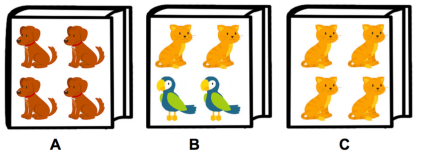
\includegraphics{figs/image-1} 

}

\caption[Example trial stimuli used in Horowitz and Frank (2015)]{Example trial stimuli used in Horowitz and Frank (2015).}\label{fig:image}
\end{figure}
\end{CodeChunk}

Horowitz, Schneider, \& Frank (in prep.) presented two hypotheses for
children's observed patterns of performance, namely, lack of quantifier
knowledge and developing inhibitory control (Horowitz et al., in prep.).
There, we reasoned that the Alternatives Hypothesis necessitates
familiarity with and ability to contrast alternatives on the quantifier
scale \(<\)\emph{none -- some -- all}\(>\); if children's quantifier
knowledge is absent or unestablished, it might lead to failures in
making an implicature. Another possible cause of children's struggles
with scalar implicatures might be that they have complete quantifier
knowledge, but are unable to inhibit an impulse to choose a more salient
alternative (e.g., choosing the book with the most cats upon hearing
``On the cover of my book, \emph{some} of the pictures are cats.'')

We explored these two hypotheses in an individual differences task,
running our scalar implicature (Horowitz \& Frank, 2015) task in
conjunction with quantifier-knowledge (D. Barner, Chow, \& Yang, 2009)
and inhibitory control (Zelazo, 2006) tasks. Overall, we found that
children's scalar implicature performance was strongly correlated with
quantifier knowledge, even when controlling for age. While inhibitory
control was strongly correlated with age, it was not related to
children's performance on the scalar implicature task (Horowitz et al.,
in prep.).

Although we found a significant relationship between quantifier
knowledge and scalar implicature comprehension, it is likely that
children's difficulties in this task has more than one source.
Importantly, in the course of conducting this individual differences
study, we observed that children who succeeded both in making a scalar
implicature and comprehending ``none'' displayed increased response
latencies. This increase in reaction time may be an important indicator
of how children are using and evaluting the salient alternatives.

It is possible that children who have a fully-established quantifier
scale must take additional time in using this information to process a
scalar implicature. This hypothesis has some support in previous
literature; Huang \& Snedeker (2009) explored online measures scalar
implicature processing through eye-tracking, and found a delay in
children's location of the referent of a scalar implicature. The exact
relationship between reaction time and accuracy using a supportive
behavioral paradigm, however, is largely unknown. Here, we explore
children's behavioral response latencies in an iPad adaptation of
Horowitz and Frank's (2015) scalar implicature task. In this study, we
explore our hypothesis that computing a scalar implicature might incur
additional processing time for children as they contrast the relevant
lexical alternatives to make a correct decision.

In our analyses, we explore overall accuracy and patterns of
performance, as in (Horowitz \& Frank, 2015; Horowitz et al., in prep.),
and find that children not only struggle in making a scalar implicature,
but also grapple with the quantifier ``none'' until fairly late in
development. In examining reaction time patterns across all quantifier
types, we find evidence of a speed-accuracy tradeoff associated with
these two quantifiers, even later in development. Finally, we use a
Drift Diffusion Model to our data to explore the source of this
increased reaction time. Overall, our findings indicate that while
quantifier knowledge is a key factor in successfully computing scalar
implicatures, using this information to successfully compute a scalar
implicature is particularly difficult, and seems to requires additional
processing.

\section{Method}\label{method}

In this study, we adapted a scalar mplicature paradigm developed by
Horowitz and Frank (2015) for the
iPad.\footnote{The full experiment can be viewed online at \texttt{https://rosemschneider.github.io/tablet\_exp/si\_tablet.html}.}
In addition to capturing detailed reaction time data, this version
included more trials, and standardized prosody across all trials, in
addition to a completely randomized
design.\footnote{All of our data, processing, experimental stimuli, and analysis code can be viewed in the version control repository for this paper at: \texttt{https://github.com/rosemschneider/SI\_tablet}.}

\subsection{Participants}\label{participants}

\begin{table}[ht]
\centering
\begin{tabular}{c c c c c } 
 \hline
 Age group & N & Mean & Median & SD \\
 \hline
 3--3.5 years & 24 & 3.27 & 3.27 & 0.14\\
 \hline
 3.5--4 years & 35 & 3.78 & 3.73 & 0.15 \\ 
 \hline
 4--4.5 years & 25 & 4.28 & 4.28 & 0.15\\
 \hline
 4.5--5 years & 30 & 4.76 & 4.76 & 0.15 \\
 \hline
 5--6.5 years & 24 & 5.55 & 5.56 & 0.36 \\
 \hline
\end{tabular}
\caption{Age demographic information for all participants.}
\label{tab:age}
\end{table}

Table \ref{tab:age} shows the breakdown of age information for all
participants. Included in analyses are 138, 138, 138, 138, 138 children
out of a planned sample of 120 participants. We ran 20 additional
children, who were excluded from analysis for low English language
exposure (\$\textless{}\$75\%) or \$\textless{}\$50\% of trials
completed. Included in our sample were 79 females and 59
males.\footnote{Based on Horowitz \& Frank (2015) and Horowitz et al.
  (in prep.), the initially planned sample size was 96 children from
  3--5 years. After collecting data from 57 participants, however, we
  observed significantly lower performance on implicature trials across
  all age groups, indicating that the iPad adaptation of the scalar
  implicature task was slightly more challenging for all children, and
  included an older age group of 24 5--6.5-year-olds.}

\subsection{Stimuli}\label{stimuli}

The general format of the task was identical to (Horowitz \& Frank,
2015), with the exception of added items for additional trials. The
study was programmed in HTML, CSS, and JavaScript, and displayed to
children on a full-sized iPad. Each trial displayed three book covers,
each containing a set of four familiar objects (Figure \ref{fig:image}).
Each trial allowed 2.5s for children to visually inspect the three book
covers, before the experiment played the trial prompt (e.g., ``On the
cover of my book, \emph{none} of the pictures are cats.''). Each trial
was randomized, with the exception that similar items were displayed
together (e.g., food, clothing). Each session involved 30 trials, with
10 trials per quantifier-type (``all'', ``some'', and ``none''). In our
randomization, quantifier triad order, items (within category), target
item, and quantifier, were randomized for all participants.

\subsection{Procedure}\label{procedure}

Sessions took place individually in a small testing room away from
either the museum or the classrooom. To familiarize children to the
iPad, each session began with the ``dot game,'' which required them to
press dots on the screen as fast as possible.

After the dot game, the experimenter introduced them to ``Hannah,'' a
cartoon character who wanted to play a guessing game with her books. The
experimenter explained that Hannah would show the child three books, and
would give \emph{one} hint about which book she had in mind. The
experimenter emphasized that Hannah would only give one hint, so they
had to listen carefully. Children then saw a practice trial with three
books featuring a refrigerator, a TV, and a couch. After 2.5s, a female
voice said ``On the cover of my book there's a TV.'' Once children
correctly made their selection, a green box appeared around the
selection. Children moved trials along at their own pace by pressing a
green button that appeared after they had made their selection.

\begin{CodeChunk}
\begin{figure}[t]
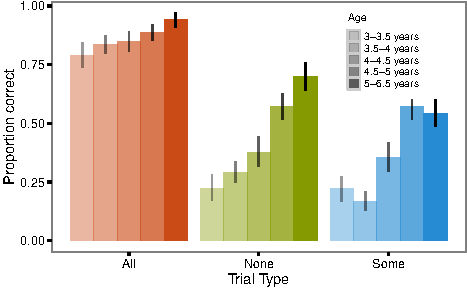
\includegraphics{figs/overall_acc-1} \caption[Children's overall accuracy for each quantifier type]{Children's overall accuracy for each quantifier type. Bars show mean performance for each age group. Error bars are 95 percent confidence intervals computed by non-parametric bootstrap.}\label{fig:overall_acc}
\end{figure}
\end{CodeChunk}

Reaction times were measured from the onset of the target word. Each
audio clip used the same three frames (e.g., ``On the cover of my book,
\emph{some} of the pictures\ldots{}'') so that prodosdy was emphasized
equally across all trials. The average length of each audio clip
(including target item phrase, e.g., ``\ldots{}are cats'') was
approximately 6s. In all, there were 270 different target items and
audio clips. Children could only make one selection. If a child was not
paying attention, or if she did not hear Hannah's prompt, the
experimenter repeated it, matching the original prosody.

\section{Results}\label{results}

In analyzing the results, we excluded any trials in which reaction time
exceeded fifteen seconds, which indicated that the child had missed the
prompt, or was not paying attention. After this initial cut, we excluded
responses outside three standard deviations of the log of mean reaction
time. This cleaning process resulted in a data loss of 85 trials
(2.14\%). Our planned analyses for this study included explorations of
accuracy, reaction time, and fitting a drift diffusion model (Ratcliff
\& Rouder, 1998) to our reaction time data.

\subsection{Accuracy}\label{accuracy}

\subsubsection{Overall accuracy}\label{overall-accuracy}

In our first planned analysis, we explored children's overall patterns
of accuracy for each quantifier type. Figure \ref{fig:overall_acc} shows
children's for each trial type, split by age group. For each age group,
we saw significantly lower accuracy for the quantifiers ``some'' and
``none'' in comparison to ``all'' in independent t-tests within each age
group (\(p\) \textless{} .01 for all tests). These results replicate our
previous findings using this paradigm (Horowitz \& Frank, 2015; Horowitz
et al., in prep.), indicating that our iPad version was a successful and
appropriate adaptation of the scalar implicature task.

One difference from the previous results was in implicature trials. We
found that children aged 3--5 years performed significantly lower on
``some'' (implicature) trials in this task in comparison with (Horowitz
et al., in prep.) in independent t-tests (\(p\) \textless{} .009 for all
tests). This difference is most likely due to the fact that our
adaptation relied strictly on verbal communication, rather than other
social and nonverbal cues.

\subsubsection{Statistical modeling}\label{statistical-modeling}

\begin{CodeChunk}
\begin{figure}[t]
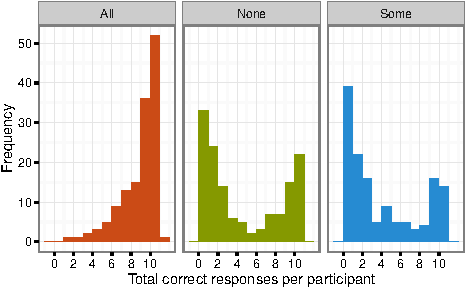
\includegraphics{figs/diptest-1} \caption[Frequency histogram of correct responses for each trial type, across all participants]{Frequency histogram of correct responses for each trial type, across all participants.}\label{fig:diptest}
\end{figure}
\end{CodeChunk}

\begin{CodeChunk}
\begin{figure*}[t]

{\centering 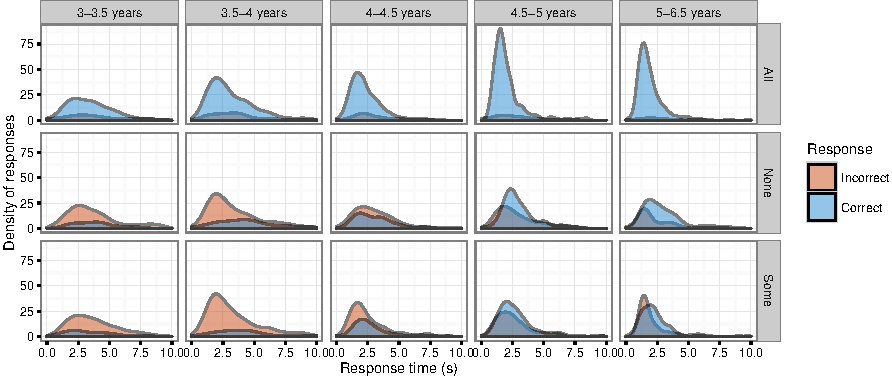
\includegraphics{figs/dense-1} 

}

\caption[Density plots of reaction times for correct and incorrect responses on each trial type, split by age]{Density plots of reaction times for correct and incorrect responses on each trial type, split by age.}\label{fig:dense}
\end{figure*}
\end{CodeChunk}

In exploring children's signficantly lower performance on ``some'' and
``none'' trials, we ran a logistic mixed effects model predicting
correct response as an interaction of age and trial type, with random
effects of trial type and
participant.\footnote{Mixed effects model fit in R using the lme4 package. The model specifications were as follows: \texttt{correct ~ age * trial type + (trial type | subject id)}.}
We found that performance was significantly lower on ``some'' (\(\beta\)
= -6.98, \(p\) \textless{} .0001) and ``none'' trials (\(\beta\) =
-9.55, \(p\) \textless{} .0001). We also found a signficant interaction
between age and trial type on ``none'' trials(\(\beta\) = 1.53, \(p\)
\textless{} .0001), indicating that children's performance with this
difficult quantifier increased with age.

\subsubsection{Correlation between ``some'' and
``none''}\label{correlation-between-some-and-none}

In previous research, a strong correlation has been found on children's
performance with the quantifiers ``some'' and ``none'' (Horowitz \&
Frank, 2015; Horowitz et al., in prep.). Figure \ref{fig:diptest} shows
distributions of correct responses for all trial types. Once again, we
found correlated performance between these two quantifiers (\(r\) =
0.49, \(p\) \textless{} .0001). In running Hartigan's diptest for
bimodality on these two quantifiers, we found significant bimodal
distributions for ``some'' (\(D\) = 0.08, \(p\) \textless{} .0001) and
``none'' trials (\(D\) = 0.11, \(p\) \textless{} .0001). While the
diptest also signficantly rejected unimodality for ``all'' trials, this
is most likely due to the distribution's long tail. The observed
significantly bimodal performance on ``some'' and ``none'' trials,
however, indicate that while children's accuracy is significantly worse
for these quantifiers, they make responses in meaningful manner over the
course of the study. In fact, although children's performance in general
was quite low on these trials, there were a number of children who got
the majority of these trials correct (``Some'': N = 28; ``None'': N =
36).

\subsection{Reaction time analyses}\label{reaction-time-analyses}

Response latencies are a largely-unexplored aspect of children's ability
to compute scalar implicatures. We hypothesized that children's reaction
times on this task may reflect processing of a scalar prompt, and
weighing quantifier alternatives. It is possible that this measure may
provide a clue as to the nature of children's correlated struggles with
these terms. In recording reaction times, we began recording from the
onset of the target nouns. Here, we explore overall trends in reaction
times across this task, and the relationship between response latencies
and accuracy on this task.

\subsubsection{Developmental reaction time
distribution}\label{developmental-reaction-time-distribution}

Figure \ref{fig:dense} shows the density of reaction times for each
quantifier, faceted by age group and trial type. Overall, we found that
reaction time was negatively correlated with age (\emph{r} = -0.25,
\emph{p} \textless{} .0001). In exploring the relationship between
accuracy and reaction time, we found preliminary evidence of a
speed-accuracy tradeoff across all trial types. Figure \ref{fig:dense}
also shows evidence for increased response latencies associated with
correct responses for the quantifiers ``some'' and ``none''. Overall, we
found that children were largely consistent in their performance across
the course of the study in reaction time correlations between reaction
times for ``all'' and ``some'' (\emph{r} = 0.76, \emph{p} \textless{}
.0001), ``all'' and ``none'' (\emph{r} = 0.65, \emph{p} \textless{}
.0001), and ``some'' and ``none'' trials (\emph{r} = 0.7, \emph{p}
\textless{} .0001).

\begin{CodeChunk}
\begin{figure*}[t]

{\centering 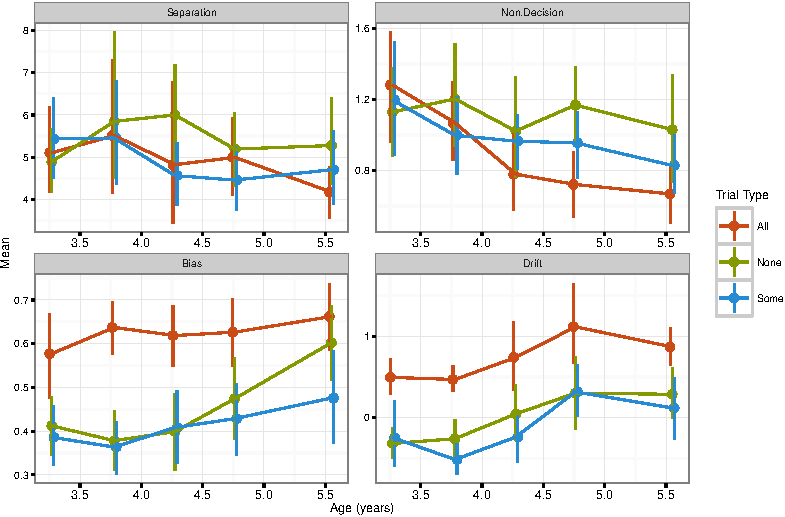
\includegraphics{figs/param_plot-1} 

}

\caption[Parameter estimates for drift diffusion model, split by age and trial type]{Parameter estimates for drift diffusion model, split by age and trial type. Error bars are 95 percent confidence intervals computed by nonparametric bootstrap.}\label{fig:param_plot}
\end{figure*}
\end{CodeChunk}

\subsubsection{Statistical modeling}\label{statistical-modeling-1}

We next turned to the relationship betwen age, reaction time, and
accuracy. Our initial hypothesis was that successfully computing
quantifiers might require additional processing time to contrast salient
alternatives. In exploring this, we ran a planned linear mixed effects
model predicting the log of reaction time as an interaction of age,
trial number, and trial type with a random effect of trial
type.\footnote{Mixed effects model fit in R using the lme4 package. The
  model specifications were as follows:
  \texttt{log(reaction time) ~ scale(age) * log(trial number) + scale(age) * trial type + (trial type | subject id)}.
  We calculated \emph{p} values by treating the \emph{t} statistic as if
  it were a \emph{z} statistic Barr, Levy, Scheepers, \& Tily (2013).}
We found a main effect of trial number, with reaction times decreasing
over the course of the study ((\(\beta\) = -0.1, \(p\) \textless{}
.00001)), but found longer reaction times on ``none'' (\(\beta\) = 0.22,
\(p\) \textless{} .00001), and ``some'' trials (\(\beta\) = 0.1, \(p\)
\textless{} .00001). Interestingly, we also found an interaction between
age and trial type, such that reaction times on ``none'' trials
increased with age relative to ``all'' trials (\(\beta\) = -0.01, \(p\)
\textless{} .02), and marginally (but not significantly) increased on
``some'' trials (\(\beta\) = 0.14, \(p\) = .38).

This interaction is particularly intriguing because in our previous
accuracy model, we found increased performance on these trial types.
While we find that older children are taking longer to respond to these
trial types, they are more likely to answer correctly, even though
reaction time is negatively correlated with age. This seems to indicate
that there is a speed-accuracy tradeoff for these quantifiers.

\subsection{Drift diffusion models}\label{drift-diffusion-models}

Our preliminary analysis of children's reaction times in this task
indicated greater response latencies associated with success on ``some''
and ``none'' trials. This suggests that children may be taking more time
to actively compare and contrast scalar alternatives as they become more
familiar with the quantifier scale. In an exploratory analysis, we fit a
drift diffusion model (DDM) to our data. A DDM can be used in behavioral
tasks to provide a more detailed view of the relationship between
accuracy and reaction time (Milosavljevic, Malmaud, Huth, Koch, \&
Rangel, 2010; Ratcliff \& Rouder, 1998).

\subsubsection{Parameter estimation}\label{parameter-estimation}

In DDM, a behavioral response (a correct or incorrect choice) is the
result of noisy data accumulation through a diffusion process
(operationalized by response time) (Ratcliff \& Rouder, 1998). Responses
have \emph{separation boundaries} that are dependent on the amount of
information needed to initate a response, and \emph{drift rate}
formalizes the rate of data accumulation (Ratcliff \& Rouder, 1998). An
additional parameter of DDM is \emph{nondecision}, which is the amount
of time between stimuli offset, and initiating response. Finally,
different responses may have a \emph{bias}, or different starting point
in the diffusion process, dependent on the stimuli (Ratcliff \& Rouder,
1998).

Although a DDM is traditionally used in two-alternative forced-choice
tasks, here we are estimating the drift process between a correct and
incorrect choice, with two options in each trial being ``incorrect,''
and only one being consistent with the target noun and quantifier. In
fitting a DDM to our data in this way, we split children by accuracy on
scalar implicature trials (high or low), and then estimated parameters
for each subject across all three trial types independently by accuracy
group. High accuracy was defined as an average of 75\% performance on
scalar implicature trials. Our goal in this exploratory analysis was to
explore whether the drift process shows differences for children who
succeed in this task versus children who fail, thus the need to estimate
parameters for high and low accuracy groups separately. We estimate
paramters using the RWiener package, and then aggregated across subjects
to obtain means and confidence intervals for each accuracy group. Figure
\ref{fig:param_plot} shows the paramter estimates for each accuracy
group, split by trial type.

In our separation boundary parameter estimates, we did not find a
significant difference of trial types for either accuracy group. This
indicates that roughly the same amount of data must be accumulated for
each trial to make a response. In nondecision estimates, ``none'' seems
to have a higher nondecision time overall, which we found with a mixed
effects model (\(\beta\) = 0.4, \(p\) =
.006).\footnote{The specifications for all parameter models are as follows (age coefficient added when specified): \texttt{Parameter Value ~ age * trial type (* age) + (1 | subject ID)}}.

While drift rates show a significant effect of accuracy, because we
estimated parameters for high and low accuracy children separately,
these are defined by the analysis. In our bias estimates, however, we
found a significant interaction between accuracy group and trial type on
``some'' trials (\(\beta\) = -0.18, \(p\) = .0013). This interaction
suggests that bias (the starting point in the diffusion process) might
be an important factor in successfully making a scalar implicature. As
another exploratory analysis, however, we included an age coefficient in
this model, and found that this interaction was no longer significant;
instead, we found a significant interaction between age, trial type
``some'', and accuracy (\(/beta\) = -0.18, \(p\) = .024). While it seems
that when accounting for age children's bias on ``some'' trials is not
affected by scalar implicature accuracy, older children in the low
accuracy group are significantly more likely to have a lower bias for
``some.''

\section{General Discussion}\label{general-discussion}

Our primary question in this study centered on whether success in making
scalar implicatures requires increased response latencies to make use of
relevant scalar alternatives. We adapted a previously validated scalar
implicature task (Horowitz \& Frank, 2015; Horowitz et al., in prep.)
for the iPad to explore the relationship between reaction time and
accuracy.

In our analyses, we replicated previous patterns of performance in
Horowitz \& Frank (2015) and Horowitz et al. (in prep.). We found that
children were overall less accurate when evaluting the quantifiers
``some'' and ``none'' in comparison to ``all,'' but that their
performance increased over development. We again found evidence of
bimodal and correlated performance on these two quantifier types,
suggesting a common source of difficulty. Additionally, we discovered in
a statistical model that although children were more likely make an
incorrect response on ``some'' and ``none'' trial, their performance on
these trials signficantly increased with age.

In our extension of this paradigm, we collected reaction time data for
these quantifier types to investigate the relationship between reaction
time and accuracy. In our reaction time analyses, we found evidence of a
speed-accuracy tradeoff, as well as an interaction between reaction time
and age, with older children taking a slightly longer time to respond to
these trials, but ultimately being more accurate. These findings
motivated our decision to fit our data to a Drift Diffusion Model.

As an exploratory analysis, we fit a DDM to our data to prediction the
relationship between reaction time and accuracy for children who succeed
in making scalar implicatures versus children who fail. While the
results are preliminary, we found some evidence that bias might be a
critical factor in success in making a scalar implicature.
Interestingly, this effect seems to be driven by age, such that older
children who fail on these trials have significantly lower bias in
comparison to ``all'' trials. It is very likely that the high
variability and wide distribution of reaction times observed in this
study contributed to the unclear findings observed in our DDM. Given
that we did see indications that bias is a significant part of
successfully making a scalar implicature, however, future work should
explore this relationship.

Our work contributes to the existing literature in utilizing a novel
method to collect accurate and detailed reaction time data on a scalar
implicature task. Response latencies are an important indicator of the
pragmatic challenges that children face in processing implicatures.
Additionally, our findings replicate previous work, providing evidence
for the appropriateness of this paradigm in targeting scalar
implicatures. Further, our larger sample size, increased number of
trials, and randomized design strengthen our analytical power, and allow
for more detailed inferences from the data. Our work supports not only
the hypthesis that children must be familiar with the quantifier scale
in order to make an implicature, but also provides preliminary evidence
that doing correctly doing so may require additional processing time.

Taken together, our work suggests that there is a meaningful
relationship between children's accuracy and reaction times in making
scalar implicatures throughout development. From our results, the
relationship between children's quantifier knowledge, processing speed,
and scalar implicature computation is unclear, and future work should
test these links more explicitly. Our work suggests, however, that
comparing a speaker's statement to possible alternatives in order to
make an implicature is an active process for children, and does seem to
result in a speed-accuracy tradeoff.

\section{Acknowledgements}\label{acknowledgements}

Special thanks to Bing Nursery School, the San Jose Children's Discovery
Museum, Veronica Cristiano, Rachel Walker, and Tamara Mekler for their
help with data collection, and to Kara Weisman and Ann Nordmeyer for
their assistance creating stimuli.

\section{References}\label{references}

\setlength{\parindent}{-0.1in} \setlength{\leftskip}{0.125in} \noindent

Barner, D., \& Bachrach, A. (2010). Inference and exact numerical
representation in early language development. \emph{Cognitive
Psychology}, \emph{60}(1), 40--62.

Barner, D., Brooks, N., \& Bale, A. (2011). Accessing the unsaid: The
role of scalar alternatives in children’s pragmatic inference.
\emph{Cognition}, \emph{118}(1), 84--93.

Barner, D., Chow, K., \& Yang, S. (2009). Finding one's meaning: A test
of the relation between quantifiers and integers in language
development. \emph{Cognitive Psychology}, \emph{58}(2), 195--219.

Barr, D. J., Levy, R., Scheepers, C., \& Tily, H. (2013). Random effects
structure for confirmatory hypothesis testing: Keep it maximal.
\emph{Journal of Memory and Language}, \emph{68}(3), 255--278.

Grice, H. (1975). \emph{Logic and conversation} (pp. 41--58).

Guasti, M., Chierchia, G., Crain, S., Foppolo, F., Gualmini, A., \&
Meroni, L. (2005). Why children and adults sometimes (but not always)
compute implicatures. \emph{Language and Cognitive Processes},
\emph{20}(5), 667--696.

Horowitz, A., \& Frank, M. C. (2015). Sources of developmental change in
pragmatic inferences about scalar terms. In \emph{Proceedings of the
37th annual conference of the cognitive science society.}

Horowitz, A., Schneider, R. M., \& Frank, M. C. (in prep.). The trouble
with quantifiers: Children's difficulties with ``some'' and ``none''.

Huang, Y. T., \& Snedeker, J. (2009). Online interpretation of scalar
quantifiers: Insight into the semantics-pragmatics interface.
\emph{Cognitive Psychology}, \emph{58}(3), 376--415.

Katsos, N., \& Bishop, D. (2011). Pragmatic tolerance: Implications for
the acquisition of informativeness and implicature. \emph{Cognition},
\emph{120}(1), 67--81.

Milosavljevic, M., Malmaud, J., Huth, A., Koch, A., \& Rangel, A.
(2010). Drift diffusion model can account for accuracy and reaction time
of value-based choices under high and low time pressure. \emph{Judgment
and Decision Making}, \emph{5}(6), 437--449.

Noveck, I. (2001). When children are more logical than adults:
Experimental investigations of scalar implicature. \emph{Cognition},
\emph{78}(2), 165--188.

Papafragou, A., \& Musolino, J. (2003). Scalar implicatures: Experiments
at the semantics-pragmatics interface. \emph{Cognition}, \emph{86}(3),
253--282.

Papafragou, A., \& Tantalou, N. (2004). Children's computation of
implicatures. \emph{Language Acquisition}, \emph{12}, 71--82.

Ratcliff, R., \& Rouder, J. (1998). Modeling response times for
two-choice decisions. \emph{Psychologial Science}, \emph{9}(5),
347--356.

Zelazo, P. D. (2006). The dimensional change card sort (dCCS): A method
of assessing executive function in children. \emph{Nature Protocols},
\emph{1}, 297--301.

\end{document}
